\chapter{General Practices}
\label{imp:general_practices}

Software development is hard and, at times, frustrating. The following
general practices should allow for greater productivity, higher
quality software and less frustration involved in the process of creating it.

\section{Documenting Functions}
When writing code, it is valuable to spend time making sure the
code is readable. One way of increasing readability is to provide comments
to non-trivial code samples. Doing this, the developer will not only
help himself, but also his peers, in later reading and understanding of the code.

When providing comments to top-level functions in C\#, it is
recommended to do so by using XML comments as seen in
\cref{fig:xml_comments_example}. By structuring the comments above a
corresponding top-level function, other software can present nicely
viewable code documentation, as seen on \cref{fig:hoverDoc}.

\begin{lstlisting}[caption = {Example of XML-comments on top of C\# function.}, label={fig:xml_comments_example}]
/// <summary>
/// Gets list of unique tracks from JSON
/// </summary>
/// <param name="jsonCode">JSON collection of tracks</param>
/// <returns>List of tracks contained in JSON</returns>
private List<Track> GetTracks(JToken jsonCode) {
\end{lstlisting}

\begin{figure}[hbtp]
  \centering
  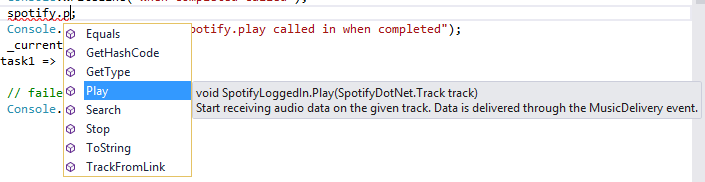
\includegraphics[width=1\linewidth]{hoverDoc}
  \caption{Example of documentation showing in Visual Studio.}\label{fig:hoverDoc}
\end{figure}